\documentclass{beamer}
\usepackage[latin1]{inputenc}

\usetheme{Madrid}
\usecolortheme{default}
\usepackage{amsmath}
\usepackage{amssymb,amsfonts,amsthm}
\usepackage{txfonts}
\usepackage{tkz-euclide}
\usepackage{listings}
\usepackage{adjustbox}
\usepackage{array}
\usepackage{tabularx}
\usepackage{gvv}
\usepackage{lmodern}
\usepackage{circuitikz}
\usepackage{tikz}
\usepackage{graphicx}
\usepackage{gensymb}
\usepackage{physics}

\setbeamertemplate{page number in head/foot}[totalframenumber]

\usepackage{tcolorbox}
\tcbuselibrary{minted,breakable,xparse,skins}



\definecolor{bg}{gray}{0.95}
\DeclareTCBListing{mintedbox}{O{}m!O{}}{%
  breakable=true,
  listing engine=minted,
  listing only,
  minted language=#2,
  minted style=default,
  minted options={%
    linenos,
    gobble=0,
    breaklines=true,
    breakafter=,,
    fontsize=\small,
    numbersep=8pt,
    #1},
  boxsep=0pt,
  left skip=0pt,
  right skip=0pt,
  left=25pt,
  right=0pt,
  top=3pt,
  bottom=3pt,
  arc=5pt,
  leftrule=0pt,
  rightrule=0pt,
  bottomrule=2pt,
  toprule=2pt,
  colback=bg,
  colframe=orange!70,
  enhanced,
  overlay={%
    \begin{tcbclipinterior}
    \fill[orange!20!white] (frame.south west) rectangle ([xshift=20pt]frame.north west);
    \end{tcbclipinterior}},
  #3,
}
\lstset{
    language=C,
    basicstyle=\ttfamily\small,
    keywordstyle=\color{blue},
    stringstyle=\color{orange},
    commentstyle=\color{green!60!black},
    numbers=left,
    numberstyle=\tiny\color{gray},
    breaklines=true,
    showstringspaces=false,
}
\title{5.8.23}
\date{2nd october, 2025}
\author{Vishwambhar - EE25BTECH11025}

\begin{document}

\frame{\titlepage}
\begin{frame}{Question}
A lending library has a fixed charge for the first three days and an additional charge for each day thereafter. Sarita paid 27 rupees for seven days, while Susheela paid 21 rupees for five days. Find the fixed charge and the charge for each extra day.\\
\end{frame}

\begin{frame}{Given}
Let:\\
The cost for the first three days be $x$.\\
The additional cost be $y$.\\
Given:
\begin{align}
    \myvec{3&4}\myvec{x\\y} = 27\\
    \myvec{3&2}\myvec{x\\y} = 21
\end{align}
\end{frame}

\begin{frame}{Solving}
Solving (1) and (2):
\begin{align}
    \augvec{2}{1}{3&4&27\\3&2&21}R_2\rightarrow R_2-R_1\\
    \augvec{2}{1}{3&4&27\\0&-2&-6}R_1\rightarrow R_1+2R_2\\
    \augvec{2}{1}{3&0&15\\0&-2&-6}R_1\rightarrow \frac{1}{3}R_1;R_2\rightarrow \frac{-1}{2}R_2\\
    \augvec{2}{1}{1&0&5\\0&1&3}
\end{align}
\end{frame}

\begin{frame}{conclusion}
The charge for the first three days is 5.\\
The additional charge is 3.
\end{frame}

\begin{frame}[fragile]
    \frametitle{C Code}
    \begin{lstlisting}
#include<stdio.h>

void get_data(double *out_data){
    out_data[0] = 3;
    out_data[1] = 4;
    out_data[2] = 3;
    out_data[3] = 2;
    out_data[4] = 27;
    out_data[5] = 21;
} 
    \end{lstlisting}
\end{frame}

\begin{frame}[fragile]
    \frametitle{Python Code 1}
    \begin{lstlisting}
import ctypes as ct
import numpy as np

def get_data():
    lib = ct.CDLL("./problem.so")
    points = ct.c_double*6
    lib.get_data.argtypes = [ct.POINTER(ct.c_double)]

    data = points()

    lib.get_data(data)

    A = np.array([[data[0],data[1]],
                  [data[2],data[3]]])
    \end{lstlisting}
\end{frame}

\begin{frame}[fragile]
    \frametitle{Python Code 1}
    \begin{lstlisting}
    Ainv = np.linalg.inv(A)

    C = np.dot(Ainv, B)

    
    E = np.array([data[0], data[1]])
    F = np.array([data[2], data[3]])
    M = B.ravel()
    D = C.ravel()
    
    return D, M, E, F
    \end{lstlisting}
\end{frame}

\begin{frame}[fragile]
    \frametitle{Python Code 2}
    \begin{lstlisting}
import matplotlib.pyplot as plt
from call import get_data
import numpy as np

D, M, E, F = get_data()

x = np.linspace(-10, 10, 200)
y = ((M[0])/E[1]) - ((E[0]*x)/E[1])

X = np.linspace(-10, 10, 200)
Y = ((M[1])/F[1]) - ((F[0]*X)/F[1])

plt.plot(x, y, color = 'blue')
plt.plot(X, Y, color = 'blue')
plt.plot(D[0], D[1], 'ro')
    \end{lstlisting}
\end{frame}

\begin{frame}[fragile]
    \frametitle{Python Code 2}
    \begin{lstlisting}
plt.text(-6.37, 19.98, "3x+2y=21", fontsize = 10, color = 'black')
plt.text(-9.68, 13.94, "3x+4y=27", fontsize = 10, color = 'black')
plt.text(5.1, 3.1, "(5,3)", fontsize = 10, color = 'black')
plt.axvline(x=0, color = 'black', linewidth = 1)
plt.axhline(y = 0, color = 'black', linewidth = 1)

plt.xlabel("X-axis")
plt.ylabel("Y-axis")
plt.axis("equal")
plt.grid(True)
plt.savefig('../figs/plot.png')
plt.show()   \end{lstlisting}
\end{frame}

\begin{frame}{Plot}
    \begin{figure}
        \centering
        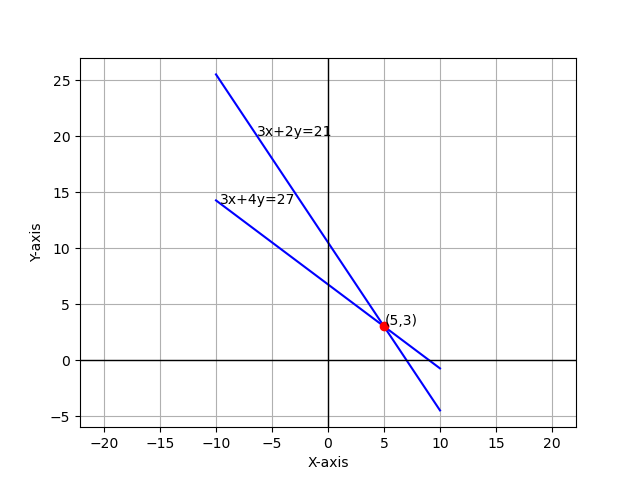
\includegraphics[width=0.5\columnwidth]{../figs/plot.png}
        \caption{Plot of given system of equations}
        \label{fig:fig}
    \end{figure}
\end{frame}
\end{document}
